\documentclass{sicnuthesis}

%在sicnuthesis模板中下面都相当于在定义学校那个丑爆的封面

\graphicspath{{images/}}


\title{题目}
\author{长者}
\school{电机系}
\major{长寿学}
\class{1926级8班}
\studentid{19890604}
\tutor{人生经验丰富的蟾蜍}
\date{1926年8月}

\begin{document}

\frontmatter %页码设为罗马数字

\maketitle

\newpage

\begin{abstractch}
    摘要是对论文内容不加注释和评论的简短陈述,要求扼要说明研究工作的目的、主要内容、研究结果、结论、
    科学意义或应用价值等,是一篇具有独立性和完整性的短文。摘要中不宜使用公式、
    图表以及非公知公用的符号和术语,不标注引用文献编号。

    摘要内容应在200~400字左右,用宋体小四号字书写。摘要内容后空两行书写“关键词”。
    毕业论文、毕业设计行与行之间、段落和层次标题以及各段落之间均为1.5倍行距。
\end{abstractch}

\vspace{1cm}

\begin{keywordsch}
    关键词1;关键词2;关键词3(关键词是供检索使用的,主题词条应为通用技术词汇,
    不得自造关键词。关键词一般为3~8个,宋体小四号字书写,按词条的学科目录分类顺序,
    由高至低顺序排列。毕业论文、毕业设计行与行之间、段落和层次标题以及各段落之间均为1.5倍行距。
    关键词与关键词之间用“;”隔开)

    (备注:毕业论文、毕业设计摘要与关键词采用英、中两种语言书写,英文在前,中文在后)
\end{keywordsch}

\newpage

\begin{abstracten}
    Abstract abstract abstract abstract abstract abstract abstract abstract abstract abstract 
    abstract abstract abstract abstract abstract abstract abstract abstract abstract abstract 
    abstract abstract abstract abstract abstract abstract abstract abstract abstract abstract 
    abstract abstract abstract.(英文摘要内容必须与中文摘要完全对应。
    英文摘要采用Times New Roman小四号字书写,毕业论文、毕业设计行与行之间、
    段落和层次标题以及各段落之间均为1.5倍行距。)
\end{abstracten}

\vspace{1cm}

\begin{keywordsen}
    Key words;key words; key words
    (英文关键词内容必须与中文关键词完全对应。英文关键词采用Times New Roman小四号字书写,
    毕业论文、毕业设计行与行之间、段落和层次标题以及各段落之间均为1.5倍行距。
    关键词与关键词之间用“;”隔开)
\end{keywordsen}

\newpage

\tableofcontents

\vspace{1cm}


(备注:目录按2~3级标题编写“目录”二字使用黑体小二号字居中书写,隔行书写目录内容,
“摘要、Abstract、正文的一级标题、结论、参考文献、附录目录、致谢”采用黑体小四号字书写,
正文其他层次标题均采用宋体小四号字书写;“摘要、Abstract”与“正文”之间隔一行;
正文中的二级标题、三级标题相对于上一级标题均缩进二个空格书写;目录行与行之间均为1.5倍行距;
目录内容多者,正文中的二、三级标题可使用宋体五号字书写,行与行之间可采用单倍行距。
目录修改时单击目录点右键选择更新域,选择更新整个目录。之后,在“Abstract”的页码后回车加一空行。)

\newpage

\mainmatter %页码设为阿拉伯数字

\section{前言}

正文采用宋体小四号字,毕业论文、毕业设计行与行之间、段落和层次标题以及各段落之间均为1.5倍行距。

毕业论文的前言应综合评述前人工作,说明论文工作的选题目的、背景和意义、国内外文献综述以及论文所要研究的主要内容,对所研究问题的认识,以及提出问题等。前言只是文章的开头,可不写章号,也可不出现“前言”二字。

毕业设计的前言部分应说明设计的目的、意义、范围及应达到的技术要求;简述课题在国内外的发展概况及存

思想;阐述设计应解决的主要问题。

\section{一级标题}

正文采用宋体小四号字,毕业论文、毕业设计行与行之间、段落和层次标题以及各段落之间均为1.5倍行距。

\subsection{二级标题}

正文采用宋体小四号字,毕业论文、毕业设计行与行之间、段落和层次标题以及各段落之间均为1.5倍行距。

具体内容 具体内容 具体内容 具体内容 具体内容 具体内容 具体内容。\cite{cite1}

\subsubsection{三级标题}

正文采用宋体小四号字,毕业论文、毕业设计行与行之间、段落和层次标题以及各段落之间均为1.5倍行距。
关于文章中公式的具体要求如下。

\begin{equation}
e^x = 1 + \frac{x}{1!} + \frac{x^2}{2!} + \frac{x^3}{3!} + \dots, \quad II < x < I
\end{equation}

正文采用宋体小四号字,毕业论文、毕业设计行与行之间、段落和层次标题以及各段落之间均为1.5倍行距。

具体内容 具体内容 具体内容 具体内容 具体内容 具体内容 具体内容\cite{cite2}。

正文采用宋体小四号字,毕业论文、毕业设计行与行之间、段落和层次标题以及各段落之间均为1.5倍行距。

图题由图号和图名组成。图号按章编排,如第1章第一图图号为“图\ref{image}”。图题置于图下,
图注或其他说明应置于图与图题之间。图名在图号之后空一格排写,图题用黑体五号字。

具体内容 具体内容,具体内容如图\ref{image}所示。

\begin{figure}[h]
\centering

\includegraphics[width=0.33\linewidth]{image.png}
\caption{图名}
\label{image}
\end{figure}

具体内容 具体内容 具体内容 具体内容 具体内容,具体内容如\ref{diagram}所示。

\begin{figure}[h]
\centering
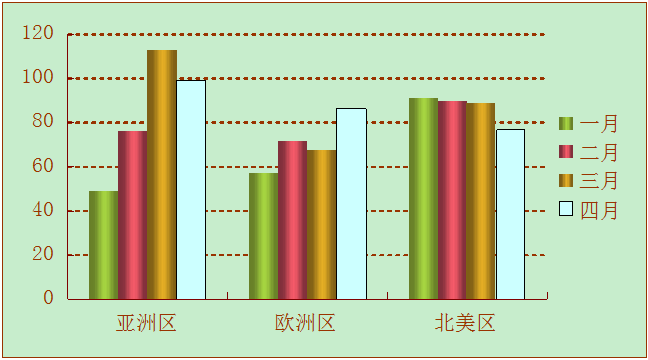
\includegraphics[width=0.66\linewidth]{diagram.png}
\caption{图名}
\label{diagram}
\end{figure}

具体内容 具体内容 具体内容,具体内容如表\ref{table1}所示。

\begin{table}
  \begin{tabular}{ c c c c c c }
    \hline
    题序层次        & 第一种 & 第二种 & 第三种    & 第四种    & 第五种    \\ \hline
    章(一级标题)  & 一、…… & 1.……  & 第一章 …… & 第一章 …… &	第一章 …… \\
    节(二级标题)  & 一、…… & 1.……  & 第一章 …… & 第一章 …… &	第一章 …… \\
    条(三级标题)  & 一、…… & 1.……  & 第一章 …… & 第一章 …… &	第一章 …… \\
    款(四级标题)  & 一、…… & 1.……  & 第一章 …… & 第一章 …… &	第一章 …… \\
    项(五级标题)  & 一、…… & 1.……  & 第一章 …… & 第一章 …… &	第一章 …… \\ \hline
  \end{tabular}
  \caption{大学本科生毕业论文、毕业设计撰写使用题序层次表}
  \label{table1}
\end{table}

论文(设计)题序层次不宜太多,不论几级标题都不能单独置于页面的最后一行,即标题排版中不能出现孤行。

毕业论文、毕业设计第一层次(章)题序和标题居中书写,其余各层次(第、条、款、项)一律沿版心左侧边线空两格安排。行与行之间、段落和层次标题以及各段落之间均为1.5倍行距。

第一层次(章)题序和标题用小二号黑体字书写;

第二层次(节)题序和标题用小三号黑体字书写;

第三层次(条)题序和标题用四号黑体字书写;

第四层次(款)题序和标题用小四号黑体字书写;

第五层次(项)以下题序和标题与第四层次同书写。

(备注:表格一般采取三线制,不加左、右边线,上、下底为粗实线(1.5磅),中间为细实线(1磅)。比较复杂的表格,可适当增加横线和竖线。表序按章编排,如第1章第一个插表序号为“表1-1”。表序与表名之间空一格,表名不允许使用标点符号。表序与表名置于表上,居中排写,采用黑体五号字。

具体内容 具体内容 具体内容,具体内容如表\ref{table2}所示。

\begin{table}
  \begin{tabular}{ c c c c c c }
    \hline
    节数   & 一班 & 二班 & 三班 & 四班 & 五班 \\ \hline
    第一节 & 语文 & 数学 & 英语 & 政治 & 化学 \\
    第二节 & 数学 & 英语 & 政治 & 化学 & 语文 \\
    第三节 & 英语 & 政治 & 化学 & 语文 & 数学 \\
    第四节 & 政治 & 化学 & 语文 & 数学 & 英语 \\
    第五节 & 化学 & 语文 & 数学 & 英语 & 政治 \\ \hline
  \end{tabular}
  \caption{**年级课程运行表}
  \label{table2}
\end{table}

\section{结论}

毕业论文的结论是对整个论文主要成果的归纳,应突出论文的创新点,以简练的文字对论文的主要工作进行评价。若不可能得出应有的结论,则需进行必要的讨论。可以在结论或讨论中提出建议、研究设想及尚待解决的问题等。

毕业设计的结论是概括说明设计的情况和价值,分析其优点和特色,有何创新,性能达到何水平,并应指出其中存在的问题和今后改进的方向。

结论要单独成页,“结论”二字采用黑体小二号字居中书写,隔行采用宋体小四号字书写具体内容,行与行之间、各段落之间均为1.5倍行距。

\newpage

%\bibliography{example}
%\bibliographystyle{unsrt}
\makebibliography{example}

至少8篇参考文献,其中至少有一篇英文文献!

\newpage

\appendix

\addcontentsline{toc}{section}{附录}

{\bf 附录一}

\vspace{1cm}

附录序号采用“附录一”、“附录二”、“附录1”、“附录2” 、“附录A”、“附录B”等,用四号黑体字左起顶格排写,其后不加标点符号,空一行书写附录内容。附录内容采用宋体小四号字书写。行与行之间、各段落之间均为1.5倍行距。

附录可有可无,当无附录内容时,此页可删除;当附录唯一时,只写“附录”即可。


\newpage

\section*{致谢}

\addcontentsline{toc}{section}{致谢}

致谢要单独成页,“致谢”二字采用黑体小二号字居中书写,隔行采用宋体小四号字书写具体内容。
行与行之间、各段落之间均为1.5倍行距。

\end{document}